
\titledquestion{Binary Tree Array Representation}

A binary tree is stored in an array using
\textbf{1-based indexing}. For a node at index $i$,
its left and right children are stored at indices
$2i$ and $2i+1$, respectively.

Index $0$ is reserved. For an array
\texttt{data[SIZE]}, valid indices are
$1,2,\ldots,\texttt{SIZE}-1$.

The height of a tree is measured in edges.

\begin{parts}

    %%%%%%%%%%%%%%%%%%%%%%%%%%%%%%%%%%%%%%%%%%%%%%%%%%%%%%%%%%
    % (a) Draw the Tree: 4 points
    %%%%%%%%%%%%%%%%%%%%%%%%%%%%%%%%%%%%%%%%%%%%%%%%%%%%%%%%%%

    \part[4]
    Suppose the occupied indices of a binary tree are

    \[
    \{1,2,3,4,5,7,8,9,14,15\}.
    \]

    \begin{enumerate}
        \item[(i)] Draw the binary tree represented
        by these indices. Label each node with its
        array index. (3 points)

        \item[(ii)] What is the height of this tree?
        (1 point)
    \end{enumerate}

    \begin{solution}

        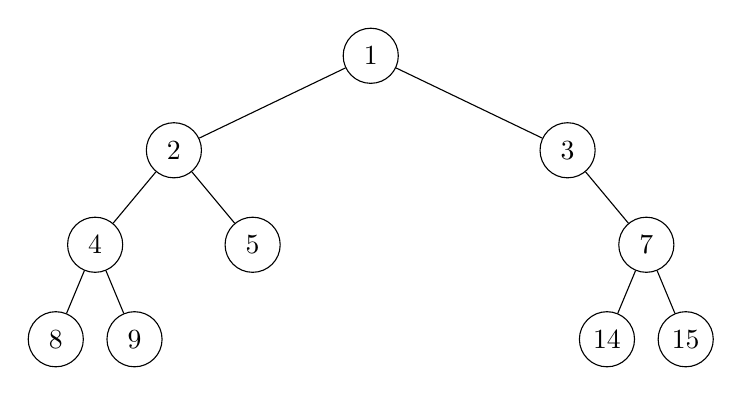
\begin{tikzpicture}[
        node/.style={circle, draw, minimum size=7mm, inner sep=1pt}
        ]
        \node[node] (n1) at (0, 0) {1};

        \node[node] (n2) at (-2.5, -1.2) {2};
        \node[node] (n3) at ( 2.5, -1.2) {3};

        \node[node] (n4) at (-3.5, -2.4) {4};
        \node[node] (n5) at (-1.5, -2.4) {5};
        \node[node] (n7) at ( 3.5, -2.4) {7};

        \node[node] (n8)  at (-4.0, -3.6) {8};
        \node[node] (n9)  at (-3.0, -3.6) {9};
        \node[node] (n14) at ( 3.0, -3.6) {14};
        \node[node] (n15) at ( 4.0, -3.6) {15};

        \draw (n1) -- (n2);
        \draw (n1) -- (n3);

        \draw (n2) -- (n4);
        \draw (n2) -- (n5);

        \draw (n3) -- (n7);

        \draw (n4) -- (n8);
        \draw (n4) -- (n9);

        \draw (n7) -- (n14);
        \draw (n7) -- (n15);
        \end{tikzpicture}

        Height of the tree is $3$.
    \end{solution}


    %%%%%%%%%%%%%%%%%%%%%%%%%%%%%%%%%%%%%%%%%%%%%%%%%%%%%%%%%%
    % (b) Complete Binary Tree: 3 points
    %%%%%%%%%%%%%%%%%%%%%%%%%%%%%%%%%%%%%%%%%%%%%%%%%%%%%%%%%%

    \part[3]
    Consider a \textbf{complete binary tree} with
    exactly $12$ nodes, stored using the same
    array representation.

    \begin{enumerate}
        \item[(i)] What is the array index of the
        parent of node $12$? (1 point)

        \item[(ii)] Is node $12$ a left child or a
        right child? (1 point)

        \item[(iii)] How many leaf nodes does this
        tree have? (1 point)
    \end{enumerate}

    \begin{solution}
        \begin{enumerate}
            \item[(i)] The parent of node $12$ is at index $\lfloor 12/2 \rfloor = 6$.

            \item[(ii)] Node $12$ is a left child because $12$ is even.

            \item[(iii)] The number of leaf nodes is $12 - \lfloor 12/2 \rfloor = 6$.
        \end{enumerate}
    \end{solution}


    %%%%%%%%%%%%%%%%%%%%%%%%%%%%%%%%%%%%%%%%%%%%%%%%%%%%%%%%%%
    % (c) Array Capacity and Boundary: 5 points
    %%%%%%%%%%%%%%%%%%%%%%%%%%%%%%%%%%%%%%%%%%%%%%%%%%%%%%%%%%

    \part[5]
    Suppose a binary tree is stored in an array
    with $\texttt{SIZE}=20$.

    \begin{enumerate}

        \item[(i)] What is the maximum possible
        height of a binary tree stored in this
        array? (1 point)

        \item[(ii)] Consider a binary tree with
        $5$ nodes, where every non-leaf node has
        only a right child.

        Can this tree be stored in the given array?
        List its required indices and explain
        your answer. (2 points)

        \item[(iii)] For an arbitrary positive
        integer $n$, what is the minimum array size
        \texttt{SIZE} that guarantees every possible
        binary tree with exactly $n$ nodes can be
        represented using this indexing scheme?
        Justify your answer. (2 points)

    \end{enumerate}

    \begin{solution}
        \begin{enumerate}
            \item[(i)] The maximum possible height of a binary tree stored in an array of size $20$ is $4$.
            
            \item[(ii)] The tree is $1 \rightarrow 3 \rightarrow 7 \rightarrow 15 \rightarrow 31$. It requires indices $\{1, 3, 7, 15, 31\}$, so the tree cannot be stored in the given array.
            
            \item[(iii)] The rightmost node of a binary tree with $n$ nodes is at index $2^n - 1$. Therefore, the minimum array size \texttt{SIZE} that guarantees every possible binary tree with exactly $n$ nodes can be represented is $2^n$.
        \end{enumerate}
    \end{solution}

\end{parts}
